\section{Database Management Systems}

In this section it will be explained what is a \gls{dbms}, a brief history of the \gls{dbms}, the advantages of using a \gls{dbms}, show the differents of  \gls{dbms} models, understand what a benchmark should do on \gls{dbms} and show the benchmark tools used here.

The \glsfirst{dbms} is the software designed to assist, maintain, and use a large set of data. This software facilitates the definition, construction, manipulation, restriction, and sharing of data ~\cite{gehrke_2002}. 

The first general-purpose \gls{dbms}, designed and developed by Charles Bachman in the early 1960s ~\cite{haigh2016charles} and it was called The Integrated Data Store. It formed the basis for the data model of the network, which through the 1960s was standardized by the Conference on \gls{codasyl} and strongly influenced database system.~\cite{gehrke_2002,haigh2016charles}.

In the late 1960s, IBM developed the \gls{ims} \gls{dbms}, used even today in many major installations. \gls{ims} formed the basis for an alternative data representation framework called the hierarchical data model ~\cite{gehrke_2002}. 

\gls{dbms} soon entered all sectors of organizations allowing the implementation of comprehensive and indispensable information systems. Historically they have evolved from the hierarchical model, which had the problem of the relationship between the entities represented, for the Relational Model that solved the relationship problem between the entities represented, allowing great flexibility navigation and search of stored data ~\cite{gehrke_2002}.

Database management continues to gain importance as more and more data is
brought online and made ever more accessible through computer networking. With the global \gls{dbms} market reached an estimated value of almost 58.4 billion American dollars in 2019. The global \gls{dbms} industry is further expected to grow at a CAGR of 13.81\% between 2020 and 2025 to reach a value of almost 126.9 billion American dollars by 2025. We can't deny the importance of the \gls{dbms} on the world. mention the advantages of why we should be using an instead of other options.

The \gls{dbms} is the software that interacts with the users application programs and the database. Typically, a \gls{dbms} provides the following facilities \cite{begg}:

\begin{itemize}
    \item It allows users to define the database, through a \gls{ddl}. The \gls{ddl} allows users to specify the data types and structures and the constraints on the data to be stored in the database.
    \item It allows users to insert, update, delete, and retrieve data from the database, usually through a \gls{dml}. Having a central repository for all data and data descriptions allows the \gls{dml} to provide a general inquiry facility to this data, called a query language.
    \item It provides controlled access to the database like a security system, which prevents unauthorized users, an integrity system, which maintains the consistency of stored data etc.
\end{itemize}


\subsection{Advantages of DBMS}
\citeauthor{gehrke_2002} mention the advantages of why we should be using \gls{dbms} an instead of other options \cite{gehrke_2002}:

\begin{itemize}
\item {\textbf{Data Independence:}} Ideally, application programs should not be exposed to data representation and storage information, and the \gls{dbms} offers an abstract view of the data that hides those details.

\item{\textbf{Efficient Data Access:}}
A \gls{dbms} utilizes a range of advanced techniques to efficiently store and retrieve information.this function is particularly important, If the data is stored on external storage devices.

\item{\textbf{Data Integrity and Security:}}  A \gls{dbms} to maintain data integrity implement restrictions on data access. Also, it can enforce access control that govern what data is visible to different classes of users.

\item{\textbf{Data Administration:}} If many users share the data, major changes can be made by centralizing data administration. Experienced professionals who understand the complexities of the data being handled, and how it is used by various groups of users, may be responsible for arranging data representation to reduce duplication and fine-tuning data storage to make recovery efficient.

\item{\textbf{Concurrent Access and Crash Recovery:}} A \gls{dbms} schedules simultaneous data access in such a way that users can think of the data as being accessed by just one user at a time. In addition, the \gls{dbms} protects users against the impact of device failures.

\item{\textbf{Reduced Application Development Time:}} 
\gls{dbms} already support several common functions between different applications and also with its high level interface. This facilitates rapid application creation in accordance with the high-level interface to the data. \gls{dbms} applications are therefore likely to be more stable than equivalent stand-alone applications since the \gls{dbms} performs several significant tasks.
\end{itemize}

Even thought have that advantages, it can bring some disadvantages:

\begin{itemize}
    \item \textbf{Danger of overkill:} For small and simple applications the use of database system is often not advisable and can have a negative impact on the overall performance. 
    \item \textbf{Complexity:} Further complexity and requirements are created by a database system. This can be quite costly and demanding to supply and operate a database management system with multiple users and databases.
    \item \textbf{Costs:} With a use of database system it will create a new costs for the system itself, but also for additional hardware and the more complex handling of the system.
    \item \textbf{Higher impact of a failure:} The centralization of resources increases the vulnerability of the system. Since all users and applications rely on the availability of the \gls{dbms}, the failure of certain components can bring operations to a halt \cite{begg}.
    \item \textbf{Cost of conversion:} In some situations, the cost of the \gls{dbms} and extra hardware may be insignificant compared with the cost of converting existing applications to run on the new \gls{dbms} and hardware \cite{begg}.
\end{itemize}


Every \gls{dbms} as is own way to store data but every one is define by a data model. A data model is a collection of high-level data description constructs that hide many low-level storage details. A \gls{dbms} allows a user to define the data to be stored in terms of a data model.

%The most popular \gls{dbms} today are based on the relational data model but there is a increase on the non relational \gls{dbms}~\cite{DBR}.

\subsection{Relational Models}
 The relational data model is based on relational algebra and was proposed by \citeauthor{codd}~\cite{codd}.
    
    The Relational Model made a revolution in the way that users used it as databases, which was just the manipulation of physical structures. \citeauthor{codd} believe that adopting his vision would allow users to use a higher-level language and abstraction, not depending to specify the physical representation of data and that improved the productivity for database users~\cite{codd2}.
    
    Relational Databases have specific characteristics like the structural aspect, Support for a language at least as powerful as relational algebra, and rules to manipulate data \cite{10.1145/320107.320109}.
    
    The relational models are more know as \glsfirst{sql} databases, which \gls{sql} is the query and maintenance language used in these applications.
    
    A relational database is in simple terms, a set of tables. Each table contains data on aspects of one subject, such as a client, an order, a product, a team, or a city. Restrictions on the data in individual tables and even between tables may be set. It is possible to usefully represent how the tables are interrelated with a data model. Different attributes of the same table may or may not have the same domain \cite{bsql}.
 
    This model have a lot of cautions and one of these cautions is that we have to normalize our data. Normalization is a technique for producing a set of relations with desirable properties, given the data requirements of an enterprise. Normalization is a formal method that can be used to identify relations based on their keys and the functional dependencies among their attributes \cite{begg}.

    Other rules this model have is in their transaction, In this context, a transaction is an operation, or a chain of operations, carried out by a single user or application program that accesses or modifies the database content. A transaction is a logical work unit that brings the database from one state of consistency to another. Transactions can be successfully terminated ~\cite{begg}.  A transaction should follow the four basic properties \gls{acid} as they know which stand for the first letter of the proprieties ~\cite{10.1145/289.291}:
\begin{itemize}
    \item \textbf{Atomicity}: The transaction operations are all done or none are. It is an all or none rule.
    \item \textbf{Consistency}: A transaction must transform the database from one consistent state to another consistent state and any of states the database can be not consistent.
    \item \textbf{Isolation}: Different Transaction are independent one of other.
    \item \textbf{Durability}: After a transaction, the effect of a transaction have a permanently recorded on the database and must survive a system failure.
\end{itemize}

Nowadays, relational \gls{dbms} are the most popular in the market following the ranking made and study by DB-Ranking~\cite{DBR} the 5 market leaders in Relational \gls{dbms} are:

\begin{itemize}
    \item Oracle
    \item MySQL
    \item Microsoft SQL Server
    \item PostgreSQL
    \item IBM Db2
\end{itemize}

Even thought that IBM developed one of the first \gls{dbms}, they struggle to be most popular \gls{dbms} because of the competitiveness of this market. However with the rise in internet traffic in recent years, the volume of accumulated data is increasingly increasing to a scale of 1,000 terabytes and even 100 \gls{pb}. The scalability of \gls{sql} storage is thus being challenged~\cite{wuoverview}.

Environments because it is not easy to put different tables across different servers, since these databases are built to manage data on the same server rather than partitioning data. In addition, it may bring additional complexity to the data model when data does not easily fit into a table, which should be avoided. The query language used in these systems, as it can only deal with standardized information, can also be a problem. Moreover, conventional \gls{sql} solutions do not work well with agile modern technology development, which can require large quantities of complicated code and in some cases, even reduced performance. NoSQL solutions have become a very hot subject and alternative to \gls{sql} databases in order to solve these scalability and performance problems ~\cite{han2011survey,wuoverview}.

\subsection{Non Relational Data Models}

The early concept of \gls{nosql} was first used in 1998 by Carlo Strozz \cite{NoSQLRel28:online} that did not expose the \gls{sql} interface, though it was based on a lightweight relational mode \cite{breiefreview,nosqlchoose,wuoverview}. However, Strozzi used the term simply to distinguish his solution from other relational \gls{dbms} \cite{nosqlchoose}.

Nowadays, the term \gls{nosql} start to regain popularity with the rise of the era of Big Data \cite{nosqlchoose}. Big data was defined by Apache Hadoop in 2010 as “datasets which could not be captured, managed, and processed by general computers within an acceptable scope.”. Big data is linked to Internet companies' services and that is rising rapidly nowadays. For example, Google processes data from hundreds of \gls{pb}, Facebook produces log data of more than 10 \gls{pb} per month, or Baidu, a Chinese business, processes data from tens of \glsplural{pb} \cite{chen2014big}. Even though traditional \gls{sql} databases have proven to be highly effective, secure, and consistent in terms of structured (or relational) data storage and processing, they fall short of Big Data processing, which is characterized, among other things, by the large volume, variety, velocity, openness, lack of structure and high visualization demands \cite{nosqlchoose,https://doi.org/10.1002/cpe.3398}.

With this information, the new definition of \gls{nosql} merges as \acrlong{nosql}. This term means that any \gls{dbms} that doesn't follow all proprieties and principles of the relational models ~\cite{wuoverview,nosqlchoose,breiefreview}. ~

\gls{nosql} systems generally have six key features \cite{cattell2011scalable}:
\begin{itemize}
    \item the ability to horizontally scale “simple operation” throughput over many servers. 
    \item the ability to partition and replicate data over many servers.
    \item a simple call level interface or protocol.
    \item a weaker concurrency model than the \gls{acid} transactions of most relational \gls{sql} database system.
    \item efficient use of distributed indexes and \gls{ram} for
data storage.
    \item the ability to dynamically add new attributes to data records.
\end{itemize}

A key feature of \gls{nosql} systems is replicating and partitioning data
over many servers. This allows them to support a large number of simple read/write operations per second. This simple operation load is traditionally called \gls{oltp}, but it is also common in modern web applications \cite{cattell2011scalable}.

To guarantee the integrity data in all levels of data management, \gls{sql} implement \gls{acid} proprieties on them transitions. However, these proprieties have poor scaling. With the face of these problems, the \gls{cap} theorem arises on \gls{nosql} databases.
\acrshort{cap} was design by \citeauthor{brewer2000towards}\cite{brewer2000towards} stands for \acrlong{cap}, and this theorem consist in 3 different aspects \cite{nosqlsyed,gilbert2012perspectives}: 
\begin{itemize} 
    \item \textbf{Strong Consistency:} All clients see the same version of the data, even on updates to the dataset.
    \item \textbf{Availability:} All clients can always find at least one copy of the requested data, even if some of the machines in a cluster are down.
    \item \textbf{Partition-tolerance:} The total system keeps its characteristic even when being deployed on different servers, transparent to the client.
\end{itemize}

    \begin{figure}[h!]
    \caption{Visualization of \gls{cap} theorem.}
    \centering
    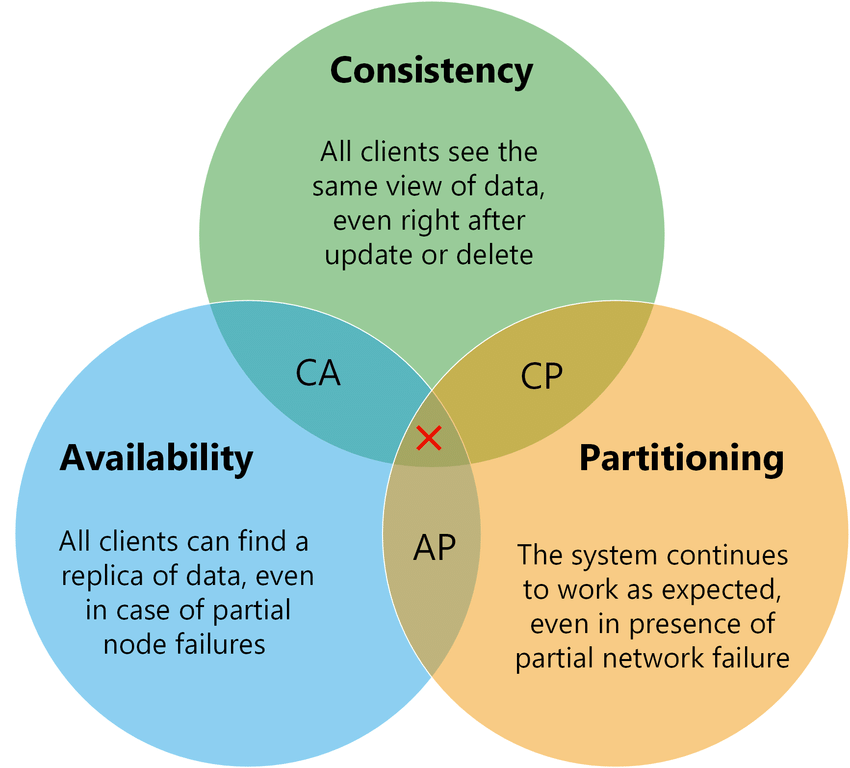
\includegraphics[width=0.65\columnwidth]{Chapters/images/Visualization-of-CAP-theorem.png}
    \label{fig:cap}
    \end{figure}

The \gls{cap} Theorem proposes that only two of the three different aspects of scaling out can be achieved fully at the same time, in figure \ref{fig:cap} we can send the 3 states that can be archive. Still systems can be improved towards the maximum proximity of the three characteristics, this state are \cite{ericcap12,cattell2011scalable,10.1145/289.291,brewer2000towards}:

\begin{itemize}
    \item \textbf{CA:} databases can only be consistency and availability at the same time if they don't have data into multiple server peers.
    \item \textbf{CP:} when working with a partitioned database, it is only possible to achieve consistency by giving up of temporary availability to have time for the partitions recovered to avoid inconsistency.
    \item \textbf{AP:} when working with partitioned data across multiple servers it is only possible to achieve total availability when giving up consistency at all times.
\end{itemize}



Many of the \gls{nosql} databases above all have loosened up the requirements on Consistency to achieve better Availability and Partitioning. This resulted in systems know as \gls{base}  \cite{base,cattell2011scalable,Startednosql}:
\begin{itemize}
    \item \textbf{Basic availability:} Each request is guaranteed a response successful or failed execution
    \item \textbf{Soft state:} The state of the system may change over time, at times without any input (for eventual consistency).
    \item \textbf{Eventual consistency:} The database may be momentarily inconsistent but will be consistent eventually.
\end{itemize}


There is been a lot of approaches and models on \gls{nosql}. This lets's create a bunch of new categories for the \gls{nosql} data models. The most popular are Key-value stores, Document stores, Graph databases, and Wide Column Stores \cite{nosqlchoose,5410700,li2013performance}.

In the next subsections, it will explain the above-mentioned \gls{nosql} models:


\subsubsection{Key-value stores}

The Key-value stores is the most simple model as the name suggest, this database only stores data as pair key and values, where stored values can be retrieved with the respective key. With this simplicity means that does any complex structured because data is organized as an array of entries but these simple systems are normally not adequate for complex applications.
These models are popular due to their simplicity, stability and efficiency, as they have, in general, linear access to the database data and usually, these models are used when you want a good cache management \cite{wuoverview,Startednosql,tiwari_2011,nosqlchoose,sabrina1448}. 

In Figure \ref{fig:KV1} shows an example of this model. If for the sets a hash map or an associative array is used as a data structure, information can be retrieved in constant time.

 \begin{figure}[H]
        \centering
        \caption{Example of a Data model of a key-value store}
        \begin{tikzpicture}
        \tikzset{
            block/.style = {draw, text width=6em, minimum height=0.7cm, rounded corners, outer sep=0pt, anchor=center, align=center},
            register/.style = {draw, text width=6em, minimum height=4ex, inner xsep=5pt, outer sep=0pt, anchor=center,align=center}, 
            map/.style={matrix of nodes, nodes=register, row sep=-\pgflinewidth, column sep=0.3cm, row 1/.style={nodes=block}},
        }
        \matrix[map] (A) {
            Key & Key & Key \\[1.5cm]
         Int & String & List\\
        };
          \foreach \i in {1,2,3}
                \draw[->] (A-1-\i) -- (A-2-\i);
        \end{tikzpicture}
                \label{fig:KV1}

    \end{figure}

It is possible to classify key-value stores into various groups. If they store data in the cache or on disk, store the keys sorted or are eventually consistent, they can be separate \cite{sabrina1448}.
 
The drawbacks are that all key-value stores share, they only support basic key/value data structures, joins are not supported and among the various implementations there is no specific query language \cite{sabrina1448}.

\subsubsection{Document stores}

Data stores, also known as document-oriented \gls{dbms}. This model is a type of database that stores uniform fields with a non-standard amount of information for each record and is distinguished by its schema-free data organization. There is no need for records or documents to have a standardized layout, and different records which have different columns. For each record, the types of individual column values can be different, and columns can have more than one value. This is possible by encapsulating documents such as JSON, XML, BSON or similar metadata technologies in a particular document type in order to compose nested semi-structured content ~\cite{nosqlchoose,sabrina1448,tiwari_2011,wuoverview,vera2015data}.

These stores organize the records into collections as a way of understanding what each document relates to. In terms of their own schema, any documents associated may be included in these collections. When dealing with data requests from a particular array, this allows to retrieve processes. A few different open-source document databases are available today but the most prominent among the available options are MongoDB and CouchDB \cite{nosqlchoose,tiwari_2011}.

In the figure \ref{fig:docexample} of a structure of a documents on a document store database.

 \begin{figure}[H]
\begin{subfigure}{.5\textwidth}
  \centering
    {\{}
    
{"EmployeeID": "SM1",}

{"FirstName" : "Anuj",}

{"LastName" : "Sharma",}

{"Age" : 45, }

{"Salary" : 10000000} 

{\}}
  \caption{Document of employee a}
  \label{fig:sfig1}
\end{subfigure}%
\begin{subfigure}{.5\textwidth}
  \centering
  {\{}
  
{"EmployeeID": "MM2",}

{"FirstName" : "Anand",}

{"Age" : 34,}

{"Salary" : 5000000,}

{"Address" : {
"Line1" : "123, 4th Street",
"City" : "Bangalore",
"State" : "Karnataka",\}
{"Projects" : [
"nosql-migration",
"top-secret-007"
]}

{\}}}}


  \caption{Document of employee b}
  \label{fig:sfig2}
\end{subfigure}
 \caption{Example of a JSON use in a data model of document store}
\label{fig:docexample}
\end{figure}


\subsubsection{Graph stores}

Graph stores are also known as graph-oriented or graph-oriented \gls{dbms}.
Databases are therefore distinct from specialized data management tools that in their implementation, use graph notions to represent data as nodes and edges in graph structures that represent relationships between nodes. They make it easy to process the data in that form and easy to calculate specific graph properties, such as the number of steps required to get from one node to another node. Graph databases allow us to enforce specifications for graph processing at the same level of query language as we use for graph data fetching without the additional abstraction layer for graph nodes and edges. This implies less overhead and more versatility and performance for graph processing~\cite{6313676,angles2008survey,nosqlchoose}.

Figure \ref{fig:graphmodel} depicts an example of a simple social network in a graph database.

\begin{figure}[H]
    \centering
    \caption{A Graph data model.}
    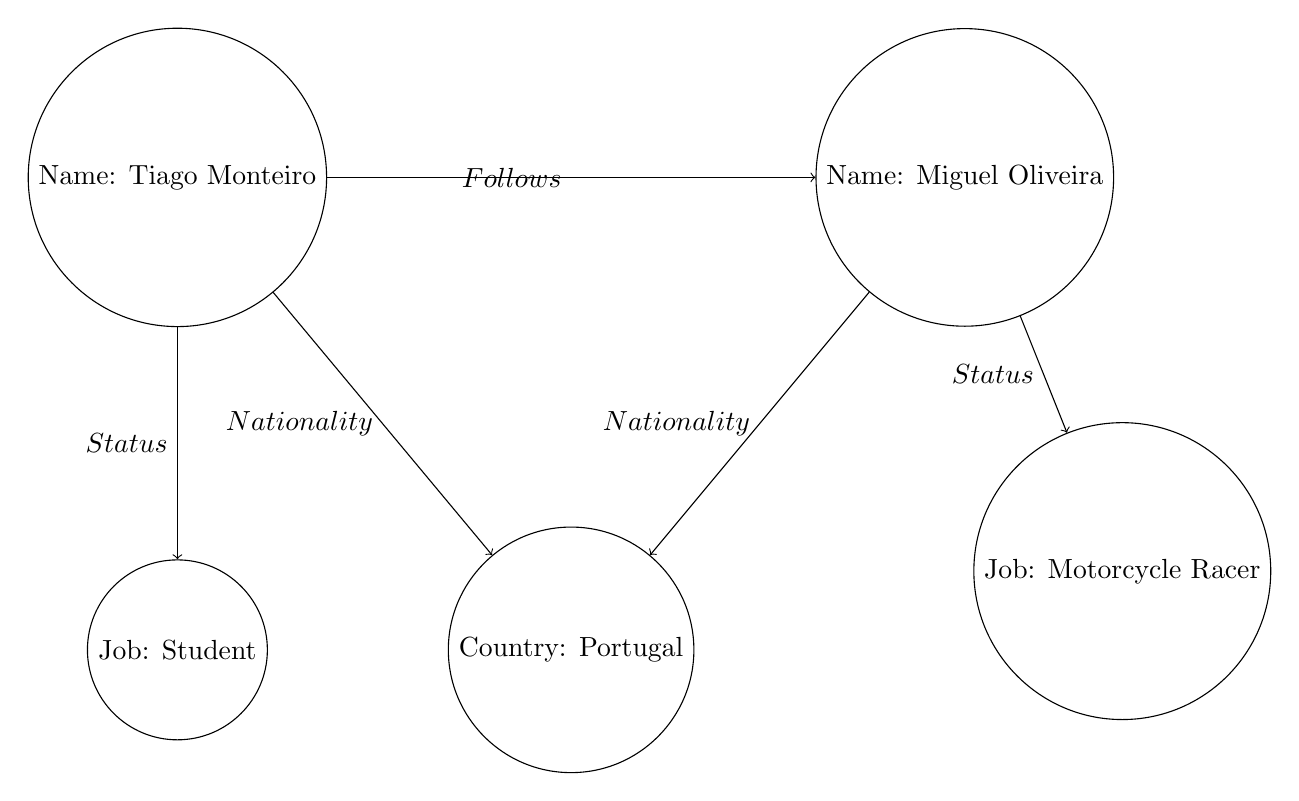
\begin{tikzpicture}
    \node[shape=circle,draw=black] (A) at (-5,3) {Name: Tiago Monteiro};
    \node[shape=circle,draw=black] (B) at (-5,-3) {Job: Student};
    \node[shape=circle,draw=black] (C) at (-0,-3) {Country: Portugal};
    \node[shape=circle,draw=black] (D) at (5,3) {Name: Miguel Oliveira
};
    \node[shape=circle,draw=black] (E) at (7,-2) {Job: Motorcycle Racer};

    

    \path [->](A) edge node[left] {$Status$} (B);
    \path [->](A) edge node[left] {$Nationality$} (C);
    \path [->](A) edge node[left] {$Follows$} (D);
    \path [->](D) edge node[left] {$Status$} (E);
    \path [->](D) edge node[left] {$Nationality$} (C);


    \end{tikzpicture}
    \label{fig:graphmodel}
\end{figure}

\subsubsection{Wide Column stores}

The first column stores appeared in 1969 \cite{abadi2009column}. In 1975 was developed the second column store and the first one with application in healthcare, for store clinical records \cite{WEYL1975279}.

Wide column stores store data in records with the capacity to carry very large numbers of complex columns, also called extensible record stores. A column-based record solution works well to act as write-optimized operations for these types of semi-structured data and it is not the case in the conventional relational DBMS that it is not optimized to write data to a smaller subset of records in order to update the records, it must read the whole set of tables. ~\cite{wuoverview,nosqlchoose}.


\subsection{Benchmark}

Benchmarks are techniques that seek to collect and compare a wide variety of activities, to achieve the best result, an objective criterion for determining which practice or software is superior in certain scenarios that the user who
is doing the simulation built. An example of popular questions is "Which domain is the best system?”. The SPECCpu benchmark ~\cite{henning2006spec}, for instance, addresses the question, "What is the best CPU?" "and the \gls{tpcc} ~\cite{council2010tpc} responds to the question, "What is the best OLTP database system?” ~\cite{benchmarkchen}.

For ~\citeauthor{gray} a domain-specific benchmark must meet four important criteria to be a useful benchmark. It must be:

\begin{itemize}
    \item \textbf{Relevant:} In performing typical operations within that problem domain, it must measure the peak performance and price/performance of systems. 
    \item \textbf{Portable:} It should be easy to implement the benchmark on many different systems and architectures.
    \item \textbf{Scaleable:}  The benchmark should apply to computer systems small and large. As computer performance and architecture evolve, it should be possible to scale the benchmark up to bigger systems and to parallel computer systems.
    \item \textbf{Simple:} The benchmark must be understandable, otherwise credibility will be lacking.
\end{itemize}



%For conducting the measurements of the energy spent, we need first a benchmark tool that can be a load generator system that can emulate a real environment in \gls{dbms}.

\subsubsection{TPC Benchmark C}
\glsfirst{tpcc} is an \gls{oltp} workload~\cite{council2010tpc}. It is a mixture of read-only and update intensive transactions that simulate the activities found in complex \gls{oltp} application environments. It does so by exercising a breadth of system components associated with such environments, which are characterized by:

\begin{itemize}
    \item The simultaneous execution of multiple transaction types that span a breadth of complexity
    \item On-line and deferred transaction execution modes
    \item Multiple on-line terminal sessions
    \item Moderate system and application execution time
    \item Significant disk input/output
    \item Transaction integrity (\gls{acid} properties)
    \item Non-uniform distribution of data access through primary and secondary keys
    \item Databases consisting of many tables with a wide variety of sizes, attributes, and relationships
    \item Contention on data access and update
\end{itemize}

While these specifications express implementation in terms of the relational data model with a traditional locking framework, any commercially available \gls{dbms}, database servers, file systems, or other data repositories offering a functionally equivalent implementation can be used to implement the database.

\gls{tpcc} uses metrics and terminology that are similar to other benchmarks originating from the TPC or others. In no way does this similarity in terminology imply that the results of \gls{tpcc} are comparable to other benchmarks. Other \gls{tpcc} results compliant with the same revision are the only benchmark results comparable to \gls{tpcc}.

The performance metric reported by \gls{tpcc} is a "business throughput" measuring the number of orders processed per minute. Multiple transactions are used to simulate the business activity of processing an order, and each transaction is subject to a response time constraint. The performance metric for this benchmark is expressed in \gls{tpmc}. 

\gls{tpcc} is accepted in the industry as the most credible transaction processing benchmark with a large body of results across all major hardware and database platforms. The highly tuned and optimized nature of the \gls{tpcc} configurations makes it the best candidate for study \gls{dbms} power consumption~\cite{powerconsumptiontppc}.

\subsubsection{HammerDB}



We decide to use HammerDB as it is a benchmark tool that can replicate the behavior of most cloud-based applications as a service, verify comprehensive performance and multiple metrics in a simple real-world environment on a virtual environment with virtual users.~\cite{hammerdb}.



HammerDB is an Open source tool and accepted tool to benchmark DBMS because of this there is a lot of studies that use and recommend HammerDB to test and/or compare different DBMS ~\cite{scalzo2018database,elgrablyanalise,knoche2016combining,benchmarkchen,ali2019persistent,yu2015design,koccak2018software,koccak2018software}. \citeauthor{elgrablyanalise} study use HammerDB to compare open-source DBMS performance like Mysql, MariaDB and Postgres \cite{elgrablyanalise}. Another study that uses Hammerdb is \citeauthor{knoche2016combining}~(\citeyear{knoche2016combining}) work that use hammerdb to test the Impact of Database Lock Contention in the \gls{tpcc} Benchmark scenario \cite{knoche2016combining}. As a final example, we have \citeauthor{koccak2018software}~(\citeyear{koccak2018software}) that use HammerDB on MySQL to have a dataset to use on his software energy consumption prediction~\cite{koccak2018software}. 


HammerDB is also used by all leading database and technology companies. It has been downloaded hundreds of thousands of times to more than 180 countries in the world and even some well know companies such as Oracle, IBM, Intel, Dell/EMC HPE, Huawei, Lenovo, and hundreds more~\cite{hammerdb}.



HammerDB is a tool that can emulate a \gls{tpcc} scenario 
and through \gls{oltp} workloads it sets up a company's sales processing environment. It reduces the testing costs by simplifying the \gls{tpcc} rules, can be modified and run on a custom environment. The above factors result in a low-cost solution, rapid deployment, and personalized benchmark test \cite{benchmarkchen,elgrablyanalise,hammerdb}. 

 Since HammerDB implements a workload based on the \gls{tpcc} specification but does not implement a complete \gls{tpcc} benchmark specification, and because of that the transaction results from HammerDB can't be compared with the official \gls{tpcc} benchmarks published. HammerDB workloads generate 2 statistics. \gls{tpm} is the transactional measurement of the specific database typically defined as the number of user commits plus the number of user rollbacks. \gls{tpm} values are database-specific cannot be compared between different types of databases. The \gls{nopm} value, on the other hand, is a performance metric independent of any particular database implementation and is the recommended primary metric to use~\cite{hammerdb}.

HammerDB currently supports Oracle, SQL Server, Db2, TimesTen, MySQL, MariaDB, PostgreSQL, Greenplum, Postgres Plus Advanced Server, Redis, and more, and can run on a variety of operating systems, being an elastic and heterogeneous tool~\cite{benchmarkchen}.

Another reason we choose him was that HammerDB is used for automated software testing \cite{hammerdb} so we can configure how many times the HammerDB will run and how many virtual users that he will use and for how long it will run, providing at the end of every execution the \gls{tpm} and the \gls{nopm}. With these numbers and the energy spent, we can have ample information to answer the RQ2, and with an adjustable number of users, it can assist in the RQ3.

